%!TEX root = main.tex
%=========================================================
\section{Evaluation}
\label{sec:evaluation}
We conduct a simulation study using Omnet++ (v5.4)~\cite{omnet} and its plug-in INET (v4.1) for wireless networks to evaluate our approach \textit{emergent overlays}.
%
This section describes the simulation set up, a micro-benchmark of broadcast protocols deployed in an heterogeneous MANET and a discussion about how our adaptive approach is positioned with existent techniques to broadcast.

\subsection{Use case and mobility model}
Figure~\ref{fig:eval:setup} depicts our experimental scenario where a crowd is carrying a single mobile device with WiFi capabilities.
%
We chose the dimensions of a soccer field as communication area with a single Point of Interest (PoI).
%
The dimensions in this region were chosen such that nodes inside it have in average three times more neighbors than those nodes out of the PoI.
%
Such density have been previously reported in real-life scenarios~\cite{versichele2012use}.
%
There is a total of 600 nodes, when the simulation starts 300 nodes are randomly positioned at the PoI and 300 nodes out of it.
%
Nodes perform truncated levy walks, that is, frequent short walks and occasional rides to distant locations where the direction of nodes motion remains invariable between walks.
%
This characterization fits well to mimic motion of humans in the context of MANETs~\cite{rhee2011levy}.
%
The velocity of every walk is chosen randomly from a fixed interval.
%
Such interval at the PoI varies between 0m/s and 0.5m/s, while out of it the velocity varies between 1.5m/s and 2m/s.
%
Nodes move freely within the whole communication area with one exception, when a node reaches the frontier of the PoI it may remain in its current region with a likelihood of 50\%.

\begin{figure}[t]
	\centering
	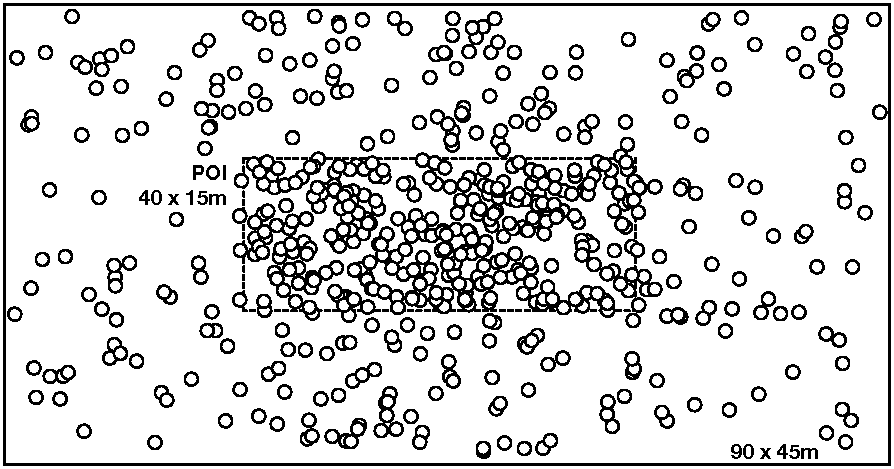
\includegraphics[width=\linewidth]{figures/setup_with_poi.pdf}
	\caption{Initial position of 600 nodes in the simulation setup.}
	\label{fig:eval:setup}
\end{figure}

\subsection{Simulation set up}
We rely on a simulation of the full network stack for MANETs, that is, the IEEE 802.11g protocol at the physical and data-link layers.
%
Ad-hoc routing in the network layer is disabled and we use BMW~\cite{tang2001mac} as MAC protocol instead of the virtual carrier sensing technique of the IEEE 802.11 standard.
%
The implementation of every broadcast protocol remains at the application layer.
%
UDP packets are used for messages with a data size of 280 bytes, which is the length of a tweet with 140 characters.
%
Each node holds a single transceiver with a transmission range of 10m, this value is commonly used in low-powered bluethoot devices and remains invariable during deployments.
%
Such transceiver works in the 2.4GHz band, with a maximum data rate of 11Mbps (default) and its power consumption per operation mode\footnote{These values correspond to the standard model of energy consumption in INET. Find more details in the official documentation (\href{https://doc.omnetpp.org/inet/api-current/neddoc/inet.physicallayer.energyconsumer.StateBasedEpEnergyConsumer.html}{link here}).} is as follows: 1mW (sleep), 5mW (listen), 10mW (receiving) and 100mW (transmitting).
%

\smallskip
\noindent
\textbf{Broadcast protocols.} Along with our implementation of emergent overlays, we provide individual implementations for controlled flooding~\cite{BroadcastStormProblem}, the overlay-based technique MPR~\cite{mpr}, an adaptive approach of controlled flooding~\cite{2001:AAR:876878.879323} and hypergossiping~\cite{hypergossiping}.
%

\smallskip
\noindent
\textbf{Individual deployments.}
%
We deploy and evaluate a single broadcast approach in the scenario depicted in Fig~\ref{fig:eval:setup}.
%
Each deployment lasts for 10 minutes and messages are sent every second by source nodes.
%
We perform 5 iterations per deployment.
%

\smallskip
\noindent
\textbf{Preconditions.}
Deployments require two inputs.
%
The first input consist in a mobility trace where nodes perform levy-walks every 0.1s.
%
At every walk we verify whether the wireless topology in the communication area is connected and keep in the mobility trace only connected topologies.
%
The second input is a list of source nodes, this selection is done randomly among those connected nodes on every wireless topology.
%
These preconditions provide a fair comparison between deployments.
%

\smallskip
\noindent
\textbf{Broadcast metrics.}
The following three metrics let us evaluate the performance of protocols:
%
\begin{itemize}
	%
	\item \emph{Coverage}. We distinguishes between two types of coverage. Reachability is the fraction of nodes that receive a message at least once. Completeness, on the other hand, is the fraction of receivers at the broadcast area of a relay node.
	%
	\item \emph{Collisions}. Number of dropped messages per node due to interference of concurrent transmissions or receptions when the transceiver is already in listening mode.
	%
	\item \emph{Network load}. Number of sent and received messages.
	%
\end{itemize} 
%

%!TEX root = main.tex

\begin{table}[t]
\setlength\tabcolsep{1pt}
\footnotesize
\centering
\newcolumntype{C}{>{\raggedright\let\newline\\\arraybackslash\hspace{0pt}}m{0.15\linewidth} }
\newcolumntype{D}{>{\centering\arraybackslash} m{0.15\linewidth} }

\newcolumntype{E}{>{\raggedleft\arraybackslash} m{0.2\linewidth} }

\begin{tabular}{CDEEE}

\toprule
	Protocol & 
	Region & 
	Avg. reach (\%) & 
	Complete (\%) & 
	Collisions (\#)
	\\
\midrule
	\multirow{3}{*}{$\text{CF}_{\text{counter}}=$3}
						& All    &  99.99  & 78.51  &  8890.00 \\ 
						& Outside &  99.98  & 100    &  3070.10  \\
						& At POI  &  100    & 35.09  &  5819.80  \\ 
\midrule
	% \multirow{3}{*}{\parbox{0.20\linewidth}{\noindent \centering MPR with $\Delta=$XX~s}} 
	\multirow{3}{0.125\linewidth}{$\text{MPR}_{\Delta}=$10s} 
						& All    &  99.90  & 94.40   & 612.90 \\ 
						& Outside &  99.90  & 97.60   & 235.20 \\
						& At POI  &  100   & 81.80   & 377.60 \\ 
\midrule
	\multirow{3}{0.125\linewidth}{$\text{MPR}_{\Delta}=$20s}
						& All    &  99.80  & 94.70   & 599.80 \\
						& Outside &  99.60  & 98   & 231.50 \\
						& At POI  &  100   & 81.50   & 368.20 \\ 
\midrule
	\multirow{3}{0.125\linewidth}{$\text{MPR}_{\Delta}=$30s} 	
						& All    &  99.30  & 95   & 621.60 \\
						& Outside &  98.70  & 98.40   & 245.20 \\
						& At POI  &  99.90  & 79.50   & 376.30 \\ 
\bottomrule
\end{tabular}
\caption{Coverage and collisions with a single protocol for the entire system, split between nodes that evolve \emph{outside} or \emph{at} the POI.}
\label{tab.conf}
\end{table}


\subsection{Microbenchmark of individual protocols}

\subsection{Quality of observables}

\subsection{Performance of emergent overlays}

\raziel{old text}

\textbf{comparison points}
\begin{itemize}
	\item 3 adaptive counter based flooding implementations with velocity as switching criterion \cite{2001:AAR:876878.879323} (coded, not tested)
	\item hypergossiping \cite{hypergossiping} (TODO)
%	\item hand-shake gossip \cite{kokuti2012adaptive} (TODO)
\end{itemize}




\textbf{Experiments}
\begin{enumerate}
	\item evaluation of the policies
	\begin{itemize}
		\item goal is to evaluate how good are the policies in deciding, and what is the impact on performance. Two main metrics are: quality of the resulting graph, and costs of the resulting hybrid system. Should include graphical representation of the selections.
	\end{itemize}
	\item comparison with related work
	\begin{itemize}
		\item running the two other approaches and comparing them to the emergent overlays (only with the best configuration found in the previous)
		\item should ideally happen on a more sophisticated setup with multiple POIs.
	\end{itemize}
\end{enumerate}


\er{
Goal for this section: show experimentally that the proposed algorithms and protocols answer the research questions set forth in the introduction.
We aim at answering the following research questions:
\begin{itemize}
	\item Does the use of a single protocol in an heterogeneously distributed MANET lead to sub-optimal performance?
	\item Is it beneficial to use different protocols for broadcast in a heterogeneously-distributed MANET, and does it reduce contention/collisions, costs, and improves overall reliability?
	\item What is the relative impact of heterogeneity in motion, and heterogeneity in placement, to the difference in performance and reliability observed in the complete MANET?
	\item What is the cost of the interoperability mechanism when a subset of the network decides to adapt and emerge an overlay in its region?
	\item Are the observables available locally to each node a good representation of the actual deployment environment of each node?
	\item How effective are the adaptation strategies in autonomously deciding on the emergence of overlays or the use of flooding-based broadcast?
\end{itemize}
The section can be structured as follows:
\begin{itemize}
	\item Experimental setup: simulator, traces, models for the nodes energy consumption, etc.
	\item Recap that we use our MAC layer
	\item Microbenchmarks with the square setup
	\item Macrobenchmarks with more complex setups, with different dense/dynamic regions over space
\end{itemize}
}



\begin{figure}[t]
	\begin{minipage}[t]{0.5\linewidth}
    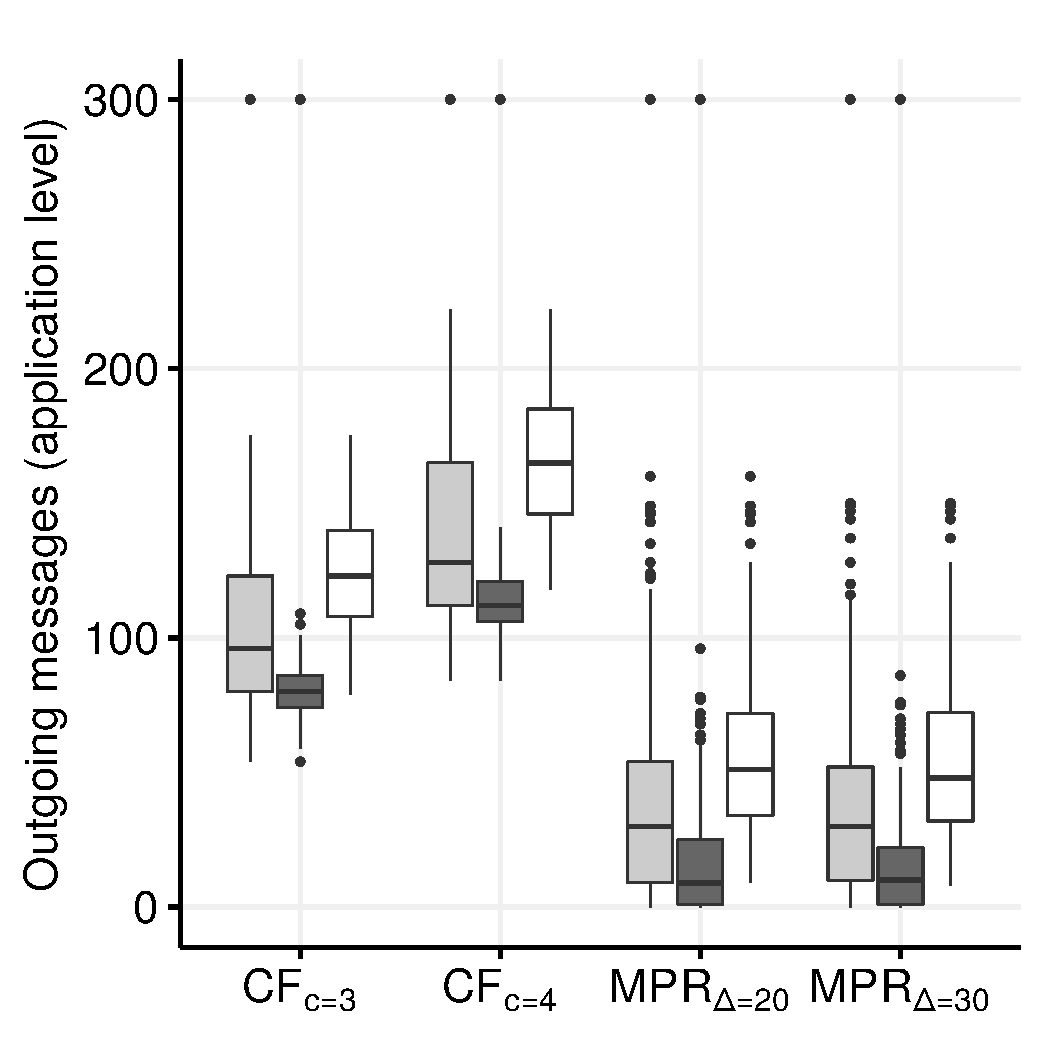
\includegraphics[width=\linewidth]{./plots/baseline-sent-msgs}
		\label{fig:eval:baseline_performance:outgoing}
	\end{minipage}%
  \hfill
	\begin{minipage}[t]{0.5\linewidth}
    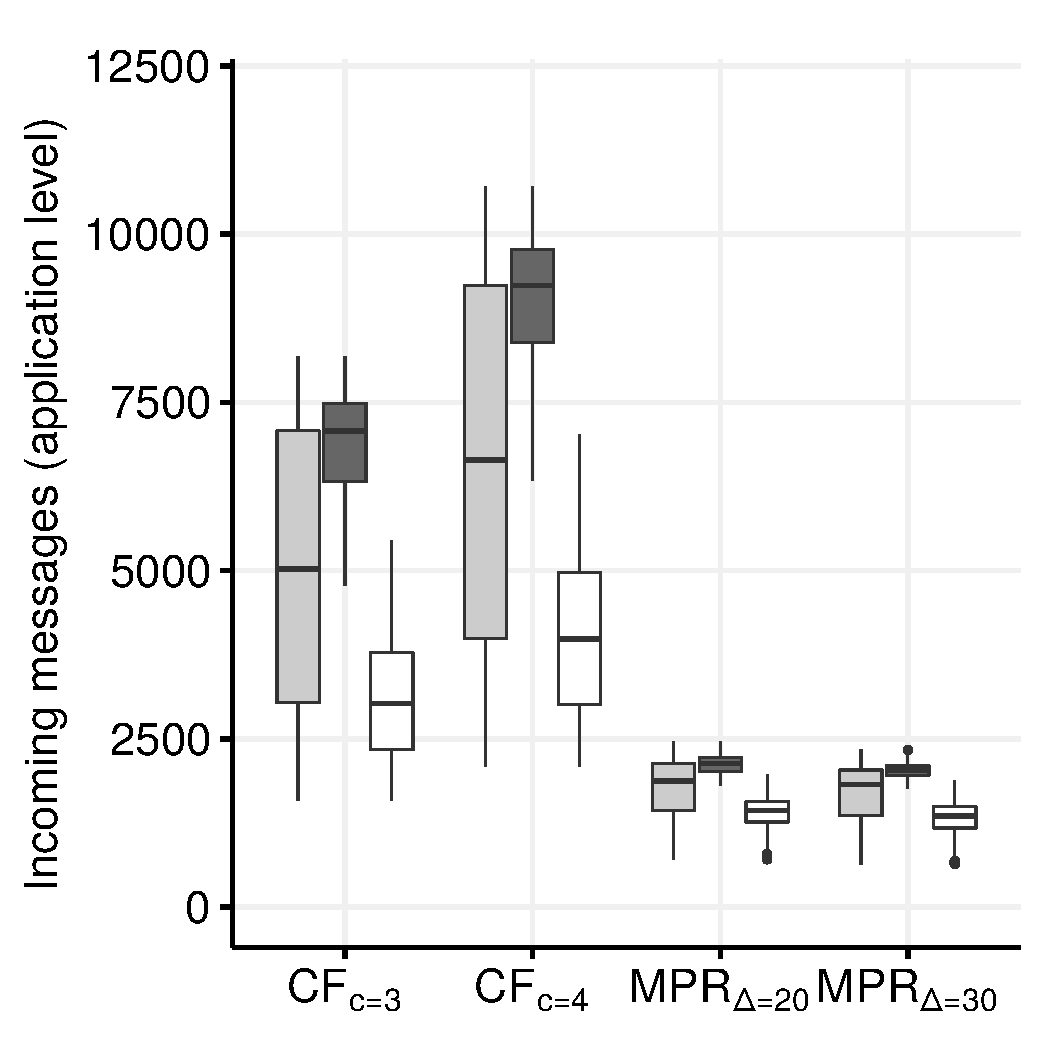
\includegraphics[width=\linewidth]{./plots/baseline-rcv-msgs}
    \label{fig:eval:baseline_performance:incoming}
	\end{minipage} 
	\caption{Performance of single-protocol deployments.}
	\label{fig:eval:baseline_performance}
\end{figure}

\begin{figure}[t]
	\begin{minipage}[t]{0.5\linewidth}
    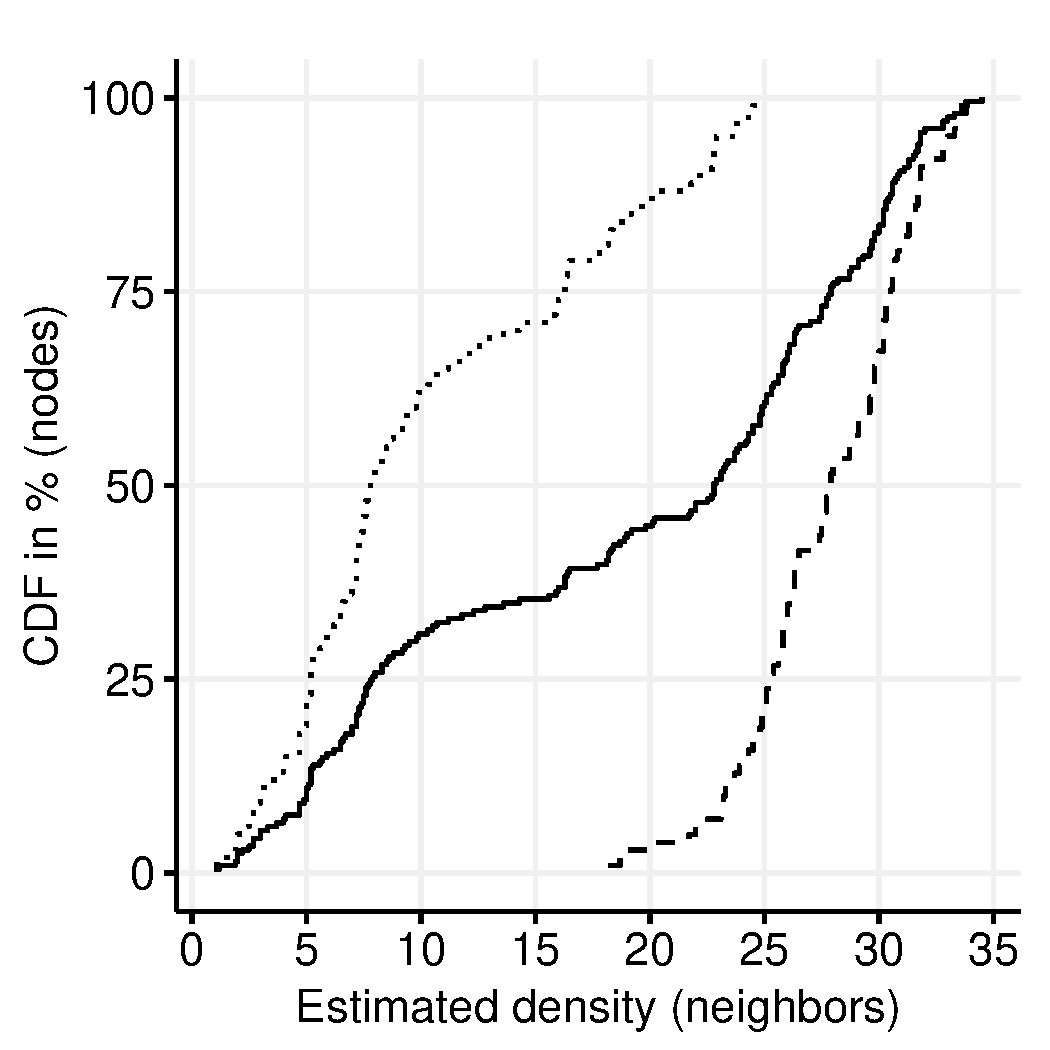
\includegraphics[width=\linewidth]{./plots/density}
		\label{fig:eval:observables:density}
	\end{minipage}%
  \hfill
	\begin{minipage}[t]{0.5\linewidth}
    
\includegraphics[width=\linewidth]{./plots/mobility}
    \label{fig:eval:observables:stability}
	\end{minipage} 
	\caption{Distribution of observables in 3 regions, out of the PoI (dotted line), at the whole communication area (solid line), and at PoI (dashed line).}
	\label{fig:eval:observables}
\end{figure}

